\renewcommand{\theequation}{\theenumi}
\begin{enumerate}[label=\thesection.\arabic*.,ref=\thesection.\theenumi]
\numberwithin{equation}{enumi}

\item 
\begin{align}
\frac{3x-4}{2} \geq \frac{x+1}{4} - 1
\\
\frac{3x-4}{2}-\frac{x+1}{4} \geq -1
\end{align}
\item Make RHS positive by multiplying with -1 on both sides , Inequality changes.
\begin{align}
-\frac{3x-4}{2}+\frac{x+1}{4} \leq 1
\end{align}
\item Convert $\leq$ sign to = sign by adding slack variable s on the LHS such that s is non-negative , That is
\begin{align}
s \geq 0
\implies -\frac{3x-4}{2}+\frac{x+1}{4} + s = 1
\\
\implies -5x+9+4s=4
\\
\implies x=1+\frac{4s}{5}
\\
\implies x \geq 1
\end{align}

The following code marks the solution of inequality on numberline as shown in figure \ref{fig:ineq_py}
\begin{lstlisting}
codes/line/ineq/ineq.py
\end{lstlisting}
\begin{figure}[!ht]
\centering
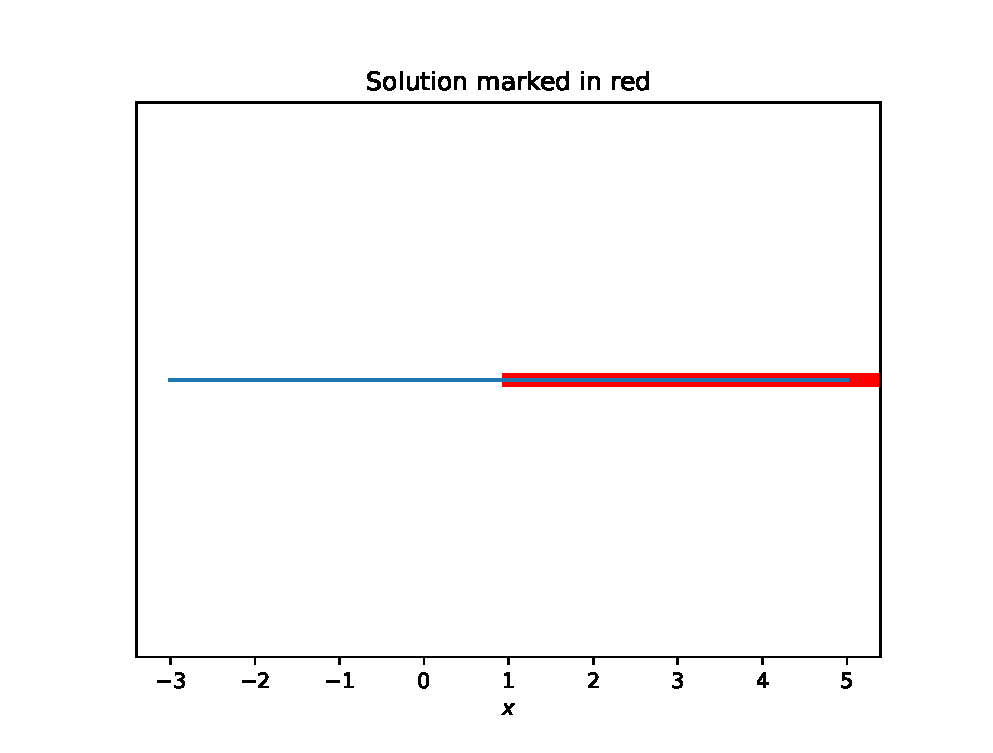
\includegraphics[width=\columnwidth]{./codes/line/ineq/pyfigs/ineq.eps}
\caption{Solution of the inequality}
\label{fig:ineq_py}
\end{figure}

\end{enumerate}
